\documentclass[]{article}
\usepackage{lmodern}
\usepackage{amssymb,amsmath}
\usepackage{ifxetex,ifluatex}
\usepackage{fixltx2e} % provides \textsubscript
\ifnum 0\ifxetex 1\fi\ifluatex 1\fi=0 % if pdftex
  \usepackage[T1]{fontenc}
  \usepackage[utf8]{inputenc}
\else % if luatex or xelatex
  \ifxetex
    \usepackage{mathspec}
  \else
    \usepackage{fontspec}
  \fi
  \defaultfontfeatures{Ligatures=TeX,Scale=MatchLowercase}
\fi
% use upquote if available, for straight quotes in verbatim environments
\IfFileExists{upquote.sty}{\usepackage{upquote}}{}
% use microtype if available
\IfFileExists{microtype.sty}{%
\usepackage{microtype}
\UseMicrotypeSet[protrusion]{basicmath} % disable protrusion for tt fonts
}{}
\usepackage[margin=1in]{geometry}
\usepackage{hyperref}
\hypersetup{unicode=true,
            pdftitle={ExamenParcial},
            pdfauthor={Yalidt Diaz - 141394; Bruno Gonzalez - 150370},
            pdfborder={0 0 0},
            breaklinks=true}
\urlstyle{same}  % don't use monospace font for urls
\usepackage{color}
\usepackage{fancyvrb}
\newcommand{\VerbBar}{|}
\newcommand{\VERB}{\Verb[commandchars=\\\{\}]}
\DefineVerbatimEnvironment{Highlighting}{Verbatim}{commandchars=\\\{\}}
% Add ',fontsize=\small' for more characters per line
\usepackage{framed}
\definecolor{shadecolor}{RGB}{248,248,248}
\newenvironment{Shaded}{\begin{snugshade}}{\end{snugshade}}
\newcommand{\AlertTok}[1]{\textcolor[rgb]{0.94,0.16,0.16}{#1}}
\newcommand{\AnnotationTok}[1]{\textcolor[rgb]{0.56,0.35,0.01}{\textbf{\textit{#1}}}}
\newcommand{\AttributeTok}[1]{\textcolor[rgb]{0.77,0.63,0.00}{#1}}
\newcommand{\BaseNTok}[1]{\textcolor[rgb]{0.00,0.00,0.81}{#1}}
\newcommand{\BuiltInTok}[1]{#1}
\newcommand{\CharTok}[1]{\textcolor[rgb]{0.31,0.60,0.02}{#1}}
\newcommand{\CommentTok}[1]{\textcolor[rgb]{0.56,0.35,0.01}{\textit{#1}}}
\newcommand{\CommentVarTok}[1]{\textcolor[rgb]{0.56,0.35,0.01}{\textbf{\textit{#1}}}}
\newcommand{\ConstantTok}[1]{\textcolor[rgb]{0.00,0.00,0.00}{#1}}
\newcommand{\ControlFlowTok}[1]{\textcolor[rgb]{0.13,0.29,0.53}{\textbf{#1}}}
\newcommand{\DataTypeTok}[1]{\textcolor[rgb]{0.13,0.29,0.53}{#1}}
\newcommand{\DecValTok}[1]{\textcolor[rgb]{0.00,0.00,0.81}{#1}}
\newcommand{\DocumentationTok}[1]{\textcolor[rgb]{0.56,0.35,0.01}{\textbf{\textit{#1}}}}
\newcommand{\ErrorTok}[1]{\textcolor[rgb]{0.64,0.00,0.00}{\textbf{#1}}}
\newcommand{\ExtensionTok}[1]{#1}
\newcommand{\FloatTok}[1]{\textcolor[rgb]{0.00,0.00,0.81}{#1}}
\newcommand{\FunctionTok}[1]{\textcolor[rgb]{0.00,0.00,0.00}{#1}}
\newcommand{\ImportTok}[1]{#1}
\newcommand{\InformationTok}[1]{\textcolor[rgb]{0.56,0.35,0.01}{\textbf{\textit{#1}}}}
\newcommand{\KeywordTok}[1]{\textcolor[rgb]{0.13,0.29,0.53}{\textbf{#1}}}
\newcommand{\NormalTok}[1]{#1}
\newcommand{\OperatorTok}[1]{\textcolor[rgb]{0.81,0.36,0.00}{\textbf{#1}}}
\newcommand{\OtherTok}[1]{\textcolor[rgb]{0.56,0.35,0.01}{#1}}
\newcommand{\PreprocessorTok}[1]{\textcolor[rgb]{0.56,0.35,0.01}{\textit{#1}}}
\newcommand{\RegionMarkerTok}[1]{#1}
\newcommand{\SpecialCharTok}[1]{\textcolor[rgb]{0.00,0.00,0.00}{#1}}
\newcommand{\SpecialStringTok}[1]{\textcolor[rgb]{0.31,0.60,0.02}{#1}}
\newcommand{\StringTok}[1]{\textcolor[rgb]{0.31,0.60,0.02}{#1}}
\newcommand{\VariableTok}[1]{\textcolor[rgb]{0.00,0.00,0.00}{#1}}
\newcommand{\VerbatimStringTok}[1]{\textcolor[rgb]{0.31,0.60,0.02}{#1}}
\newcommand{\WarningTok}[1]{\textcolor[rgb]{0.56,0.35,0.01}{\textbf{\textit{#1}}}}
\usepackage{longtable,booktabs}
\usepackage{graphicx,grffile}
\makeatletter
\def\maxwidth{\ifdim\Gin@nat@width>\linewidth\linewidth\else\Gin@nat@width\fi}
\def\maxheight{\ifdim\Gin@nat@height>\textheight\textheight\else\Gin@nat@height\fi}
\makeatother
% Scale images if necessary, so that they will not overflow the page
% margins by default, and it is still possible to overwrite the defaults
% using explicit options in \includegraphics[width, height, ...]{}
\setkeys{Gin}{width=\maxwidth,height=\maxheight,keepaspectratio}
\IfFileExists{parskip.sty}{%
\usepackage{parskip}
}{% else
\setlength{\parindent}{0pt}
\setlength{\parskip}{6pt plus 2pt minus 1pt}
}
\setlength{\emergencystretch}{3em}  % prevent overfull lines
\providecommand{\tightlist}{%
  \setlength{\itemsep}{0pt}\setlength{\parskip}{0pt}}
\setcounter{secnumdepth}{0}
% Redefines (sub)paragraphs to behave more like sections
\ifx\paragraph\undefined\else
\let\oldparagraph\paragraph
\renewcommand{\paragraph}[1]{\oldparagraph{#1}\mbox{}}
\fi
\ifx\subparagraph\undefined\else
\let\oldsubparagraph\subparagraph
\renewcommand{\subparagraph}[1]{\oldsubparagraph{#1}\mbox{}}
\fi

%%% Use protect on footnotes to avoid problems with footnotes in titles
\let\rmarkdownfootnote\footnote%
\def\footnote{\protect\rmarkdownfootnote}

%%% Change title format to be more compact
\usepackage{titling}

% Create subtitle command for use in maketitle
\providecommand{\subtitle}[1]{
  \posttitle{
    \begin{center}\large#1\end{center}
    }
}

\setlength{\droptitle}{-2em}

  \title{ExamenParcial}
    \pretitle{\vspace{\droptitle}\centering\huge}
  \posttitle{\par}
    \author{Yalidt Diaz - 141394 \\ Bruno Gonzalez - 150370}
    \preauthor{\centering\large\emph}
  \postauthor{\par}
      \predate{\centering\large\emph}
  \postdate{\par}
    \date{7/10/2019}


\begin{document}
\maketitle

\hypertarget{examen-parcial}{%
\subsection{EXAMEN PARCIAL}\label{examen-parcial}}

\hypertarget{tablas-de-conteos-y-bootstrap}{%
\paragraph{1. Tablas de conteos y
bootstrap}\label{tablas-de-conteos-y-bootstrap}}

En la sección de visualización vimos un ejemplo de tabla de perfiles.

En este ejercicio construiremos intervalos de confianza para una tabla
de perfiles usando bootstrap. Usaremos los datos de tomadores de te (del
paquete @factominer):

Nos interesa ver qué personas compran té suelto (\texttt{unpacked}), y
de qué tipo (\texttt{Tea}). Empezamos por ver las proporciones que
compran té según su empaque (en bolsita o suelto):

\begin{longtable}[]{@{}lrr@{}}
\toprule
how & n & \%\tabularnewline
\midrule
\endhead
tea bag & 170 & 57\tabularnewline
tea bag+unpackaged & 94 & 31\tabularnewline
unpackaged & 36 & 12\tabularnewline
\bottomrule
\end{longtable}

La tabla de arriba es poco informativa, buscamos comparar grupos, por
ejemplo, queremos investigar si hay diferencias en los patrones de
compra (en términos de precio o marca) dependiendo del tipo de té que
consumen.

\begin{longtable}[]{@{}lrrr@{}}
\toprule
price & tea bag & tea bag+unpackaged & unpackaged\tabularnewline
\midrule
\endhead
p\_branded & 41 & 21 & 14\tabularnewline
p\_cheap & 3 & 1 & 3\tabularnewline
p\_private label & 9 & 4 & 3\tabularnewline
p\_unknown & 6 & 1 & 0\tabularnewline
p\_upscale & 8 & 20 & 56\tabularnewline
p\_variable & 32 & 52 & 25\tabularnewline
\bottomrule
\end{longtable}

Para facilitar la comparación podemos calcular \emph{perfiles columna}.
Comparamos cada una de las columnas con la columna marginal (la tabla de
tipo de estilo de té):

\begin{longtable}[]{@{}lrrrr@{}}
\toprule
price & tea bag & tea bag+unpackaged & unpackaged &
promedio\tabularnewline
\midrule
\endhead
p\_private label & 0.72 & -0.22 & -0.49 & 5\tabularnewline
p\_unknown & 0.72 & -0.72 & -1.00 & 4\tabularnewline
p\_branded & 0.62 & -0.16 & -0.45 & 25\tabularnewline
p\_cheap & 0.30 & -0.53 & 0.23 & 2\tabularnewline
p\_variable & -0.12 & 0.44 & -0.31 & 36\tabularnewline
p\_upscale & -0.71 & -0.28 & 0.98 & 28\tabularnewline
\bottomrule
\end{longtable}

Leemos esta tabla como sigue: por ejemplo, los compradores de té suelto
(\texttt{unpacked}) compran té fino (\texttt{upscale}) a una tasa casi
el doble (0.98) que el promedio.

También podemos graficar como:

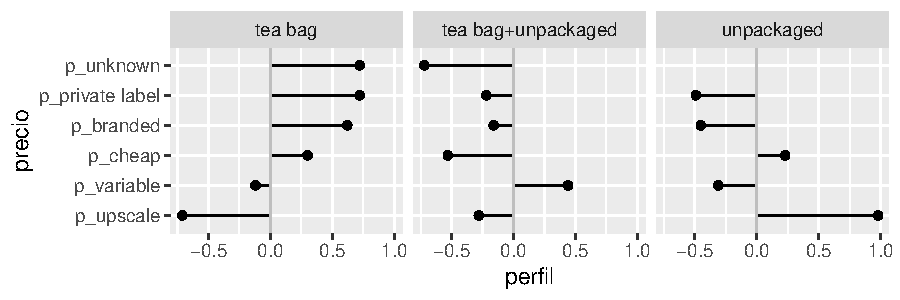
\includegraphics{ExamenParcial_files/figure-latex/perfiles_grafica-1.pdf}

\textbf{Observación}: hay dos maneras de construir la columna promedio:
tomando los porcentajes sobre todos los datos, o promediando los
porcentajes de las columnas como en este ejemplo.

\begin{enumerate}
\def\labelenumi{\arabic{enumi}.}
\tightlist
\item
  Utiliza bootstrap para crear intervalos de confianza sobre los
  perfiles de la última tabla.
\end{enumerate}

Primero definimos la funcion bootstrap, la cual seleccionará las
muestras aleatoreas con reemplazo, y posterior mente calcula la
estadística de interés, que en este caso son los \emph{perfiles
columna}.

\begin{Shaded}
\begin{Highlighting}[]
\NormalTok{perfiles_boot <-}\StringTok{ }\ControlFlowTok{function}\NormalTok{(x)\{}
\NormalTok{  m <-}\StringTok{ }\KeywordTok{sample_n}\NormalTok{(x, }\DataTypeTok{size =}  \DecValTok{300}\NormalTok{ , }\DataTypeTok{replace =} \OtherTok{TRUE}\NormalTok{)}
\NormalTok{  tabla <-}\StringTok{ }\NormalTok{m }\OperatorTok\StringTok{ }
\StringTok{    }\KeywordTok{count}\NormalTok{(how, price) }\OperatorTok\StringTok{ }
\StringTok{    }\KeywordTok{group_by}\NormalTok{(how) }\OperatorTok\StringTok{ }
\StringTok{    }\KeywordTok{mutate}\NormalTok{(}\DataTypeTok{prop_price =}\NormalTok{ (}\DecValTok{100} \OperatorTok{*}\StringTok{ }\NormalTok{n }\OperatorTok{/}\StringTok{ }\KeywordTok{sum}\NormalTok{(n))) }\OperatorTok\StringTok{ }
\StringTok{    }\KeywordTok{group_by}\NormalTok{(price) }\OperatorTok\StringTok{ }
\StringTok{    }\KeywordTok{mutate}\NormalTok{(}\DataTypeTok{prom_prop =} \KeywordTok{mean}\NormalTok{(prop_price)) }\OperatorTok\StringTok{ }
\StringTok{    }\KeywordTok{mutate}\NormalTok{(}\DataTypeTok{perfil =}\NormalTok{ (prop_price }\OperatorTok{/}\StringTok{ }\NormalTok{prom_prop }\OperatorTok{-}\StringTok{ }\DecValTok{1}\NormalTok{) }\OperatorTok\StringTok{ }\KeywordTok{round}\NormalTok{(}\DecValTok{2}\NormalTok{))}
\NormalTok{  tabla}
\NormalTok{\}}
\end{Highlighting}
\end{Shaded}

Despues corremos \(B = 10000\) replicaciones Bootstrap.

\begin{Shaded}
\begin{Highlighting}[]
\NormalTok{perfiles_rep <-}\StringTok{ }\KeywordTok{rerun}\NormalTok{(}\DecValTok{10000}\NormalTok{, }\KeywordTok{perfiles_boot}\NormalTok{(tea)) }\OperatorTok\StringTok{ }\KeywordTok{bind_rows}\NormalTok{(}\DataTypeTok{.id =} \StringTok{'muestra'}\NormalTok{)}
\end{Highlighting}
\end{Shaded}

Posteriormente calculamos los errores estándard

\begin{Shaded}
\begin{Highlighting}[]
\NormalTok{perfiles_se <-}\StringTok{ }\NormalTok{perfiles_rep }\OperatorTok\StringTok{ }
\StringTok{  }\KeywordTok{group_by}\NormalTok{(how, price) }\OperatorTok\StringTok{ }
\StringTok{  }\KeywordTok{summarise}\NormalTok{(}\DataTypeTok{se =} \KeywordTok{sd}\NormalTok{(perfil))}
\end{Highlighting}
\end{Shaded}

Por último calculamos los intervalos

\begin{Shaded}
\begin{Highlighting}[]
\NormalTok{perfiles_int <-}\StringTok{ }\NormalTok{tabla }\OperatorTok\StringTok{ }
\StringTok{  }\KeywordTok{left_join}\NormalTok{(perfiles_se) }\OperatorTok\StringTok{ }
\StringTok{  }\KeywordTok{mutate}\NormalTok{(}\DataTypeTok{Int_inf =}\NormalTok{ perfil}\OperatorTok{+}\KeywordTok{qnorm}\NormalTok{(}\FloatTok{0.025}\NormalTok{)}\OperatorTok{*}\NormalTok{se, }\DataTypeTok{Int_sup =}\NormalTok{ perfil}\OperatorTok{+}\KeywordTok{qnorm}\NormalTok{(}\FloatTok{0.975}\NormalTok{)}\OperatorTok{*}\NormalTok{se)}

\KeywordTok{kable}\NormalTok{(}\KeywordTok{select}\NormalTok{(perfiles_int, how, price, perfil, Int_inf, Int_sup), }\DataTypeTok{digits =} \DecValTok{2}\NormalTok{)}
\end{Highlighting}
\end{Shaded}

\begin{longtable}[]{@{}llrrr@{}}
\toprule
how & price & perfil & Int\_inf & Int\_sup\tabularnewline
\midrule
\endhead
tea bag & p\_branded & 0.62 & 0.29 & 0.95\tabularnewline
tea bag & p\_cheap & 0.30 & -0.36 & 0.96\tabularnewline
tea bag & p\_private label & 0.72 & 0.14 & 1.30\tabularnewline
tea bag & p\_unknown & 0.72 & 0.10 & 1.34\tabularnewline
tea bag & p\_upscale & -0.71 & -0.86 & -0.56\tabularnewline
tea bag & p\_variable & -0.12 & -0.32 & 0.08\tabularnewline
tea bag+unpackaged & p\_branded & -0.16 & -0.44 & 0.12\tabularnewline
tea bag+unpackaged & p\_cheap & -0.53 & -1.11 & 0.05\tabularnewline
tea bag+unpackaged & p\_private label & -0.22 & -0.75 &
0.31\tabularnewline
tea bag+unpackaged & p\_unknown & -0.72 & -1.09 & -0.35\tabularnewline
tea bag+unpackaged & p\_upscale & -0.28 & -0.55 & -0.01\tabularnewline
tea bag+unpackaged & p\_variable & 0.44 & 0.18 & 0.70\tabularnewline
unpackaged & p\_branded & -0.45 & -0.82 & -0.08\tabularnewline
unpackaged & p\_cheap & 0.23 & -0.53 & 0.99\tabularnewline
unpackaged & p\_private label & -0.49 & -1.04 & 0.06\tabularnewline
unpackaged & p\_upscale & 0.98 & 0.68 & 1.28\tabularnewline
unpackaged & p\_variable & -0.31 & -0.62 & 0.00\tabularnewline
\bottomrule
\end{longtable}

\begin{enumerate}
\def\labelenumi{\arabic{enumi}.}
\setcounter{enumi}{1}
\tightlist
\item
  Modifica la última gráfica para representar los intervalos de
  confianza.
\end{enumerate}

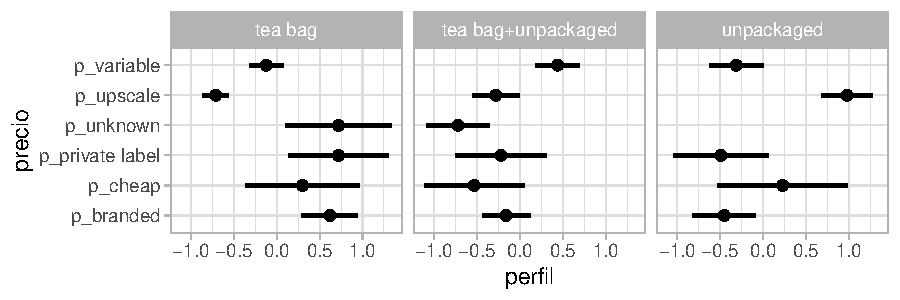
\includegraphics{ExamenParcial_files/figure-latex/perfiles_intervalos_grafica, -1.pdf}

\begin{enumerate}
\def\labelenumi{\arabic{enumi}.}
\setcounter{enumi}{2}
\tightlist
\item
  Comenta tus observaciones.
\end{enumerate}

En la categoria de ``tea bag'' la mayor tasa de compra corresponde a los
precios ``private label'' y ``unknown'' que son .72 aproximadamente, sin
embargo el intervalo deconfianza para ambdos casos es relativamente
alto, lo que le quita certidumbre a la estimación. Por otro lado, en est
misma categoría, los que tienen menor perfil de compra es
``p\_upscale'', con un intervalo muy chico lo que permite concluir con
mayor certeza que este patrón se mantiene en la población total.

En el caso de ``tea\_bag+unpackaged'' la mayor tasa de compra es a una
precio ``p\_variable'',cuyo intervalo se enceuntra entre .18 y.70, y la
menor tasa(negativa) es a precio ``p\_known''. Por útimo, en la
categoría unpackaged la mayor tasa de compra es a precio ``p\_upscale''
a una tasa de casi el doble .89 con un intervalo de confianza de .68 y
1.28, en el caso de la menor tasa de compra se obtuvó que la menor fue a
precio p\_private\_label.

En general, aquellos intervalos con mayor rango son aquellos donde hay
menos observaciones(`p\_cheap', `p\_private label',`p\_unknown'). Estos
intervalos con tanta variación y que tienen una longuitud (segmento) muy
amplia no son tan confiables, se esperaría que la longuitud fuera lo
menor posible para tener mayor certeza de que valor tomaría la variable
estimada.

En conclusión pareciera que el mejor comportamiento de compra se
desarrolla en la categoría p\_unpackaged a un precio upscale, por lo que
se recomendaría trabajar en dicho segmento, porque ahí la gente tiene un
perfil de compra mas agudo que en los demás casos.

\hypertarget{cuantificando-el-error-monte-carlo}{%
\paragraph{2. Cuantificando el error Monte
Carlo}\label{cuantificando-el-error-monte-carlo}}
\addcontentsline{toc}{paragraph}{2. Cuantificando el error Monte Carlo}

Recordemos que ante la pregunta ¿cuántas muestras bootstrap se
necesitan? el error que podemos disminuir al aumentar el número de
replicaciones es el error de Monte Carlo, y una manera de cuantificarlo
es haciendo bootstrap del bootstrap.

Retomemos el ejemplo de la media de las calificaciones de ENLACE de
español 3o de primaria en el estado de México. Nos interesa la media de
las calificaciones y usaremos el estimador \emph{plug-in}.

\begin{enumerate}
\def\labelenumi{\arabic{enumi}.}
\tightlist
\item
  Crea un intervalo del 90\% para \(\hat{\theta}\) usando los
  percentiles de la distribución bootstrap, y \(B=100\) replicaciones.
\end{enumerate}

Primero creamos la función bootstrap que genera las muestras y calcula
el parámetro, en este caso, la mediana.

\begin{Shaded}
\begin{Highlighting}[]
\NormalTok{enlace_boot <-}\StringTok{ }\ControlFlowTok{function}\NormalTok{(x,col)\{}
\NormalTok{  col <-}\StringTok{ }\KeywordTok{enquo}\NormalTok{(col)}
\NormalTok{  n <-}\StringTok{ }\KeywordTok{nrow}\NormalTok{(x)}
\NormalTok{  muestra <-}\StringTok{ }\KeywordTok{sample_n}\NormalTok{(x,n, }\DataTypeTok{replace =} \OtherTok{TRUE}\NormalTok{)}
\NormalTok{  muestra }\OperatorTok\StringTok{ }
\StringTok{    }\KeywordTok{select}\NormalTok{(}\OperatorTok{!!}\NormalTok{col) }\OperatorTok\StringTok{ }
\StringTok{    }\KeywordTok{unlist}\NormalTok{() }\OperatorTok\StringTok{ }
\StringTok{    }\KeywordTok{median}\NormalTok{()}
\NormalTok{\}}
\end{Highlighting}
\end{Shaded}

Posteriormente se hacen las \(B=100\) simulaciones bootstrap.

\begin{Shaded}
\begin{Highlighting}[]
\NormalTok{enlace_rep <-}\StringTok{ }\KeywordTok{rerun}\NormalTok{(}\DecValTok{100}\NormalTok{, }\KeywordTok{enlace_boot}\NormalTok{(enlace,esp_}\DecValTok{3}\NormalTok{))}\OperatorTok
\StringTok{  }\KeywordTok{flatten_dbl}\NormalTok{()}
\end{Highlighting}
\end{Shaded}

Por último, calculamos el intervalos usando los percentiles de la
distrubucion bootstrap.

\begin{Shaded}
\begin{Highlighting}[]
\NormalTok{en_int <-}\StringTok{ }\KeywordTok{quantile}\NormalTok{(enlace_rep, }\KeywordTok{c}\NormalTok{(}\FloatTok{0.05}\NormalTok{, }\FloatTok{0.95}\NormalTok{))}
\NormalTok{en_int}
\end{Highlighting}
\end{Shaded}

\begin{verbatim}
##  5% 95% 
## 546 549
\end{verbatim}

Las calificaciones de 3er año de primaria en el estado de México se
encuentra en un intervalo al 95\% de confianza entre 546 y 549 puntos.

\begin{enumerate}
\def\labelenumi{\arabic{enumi}.}
\setcounter{enumi}{1}
\tightlist
\item
  Podemos estimar el error estándar de Monte Carlo de los extremos de
  los intervalos (percentiles 0.05 y 0.95) haciendo bootstrap de la
  distribución bootstrap:
\end{enumerate}

\begin{itemize}
\tightlist
\item
  Selecciona muestras con reemplazo de tamaño \(B\) de la distribución
  bootstrap,
\item
  Calcula los percentiles de interés (0.05 y 0.95),
\end{itemize}

Primero construimos la función bootstrap de la distribución bootstrap

\begin{Shaded}
\begin{Highlighting}[]
\NormalTok{enlace_boot_boot <-}\StringTok{ }\ControlFlowTok{function}\NormalTok{(x)\{}
\NormalTok{  n <-}\StringTok{ }\KeywordTok{length}\NormalTok{(x)}
\NormalTok{  muestra <-}\StringTok{ }\KeywordTok{sample}\NormalTok{(x, }\DataTypeTok{size =}\NormalTok{ n, }\DataTypeTok{replace =} \OtherTok{TRUE}\NormalTok{)}
  \KeywordTok{tibble}\NormalTok{(}\DataTypeTok{SE_inf =} \KeywordTok{quantile}\NormalTok{(muestra, }\KeywordTok{c}\NormalTok{(}\FloatTok{0.025}\NormalTok{,}\FloatTok{0.975}\NormalTok{))[}\DecValTok{1}\NormalTok{], }\DataTypeTok{SE_sup =} \KeywordTok{quantile}\NormalTok{(muestra, }\KeywordTok{c}\NormalTok{(}\FloatTok{0.025}\NormalTok{,}\FloatTok{0.975}\NormalTok{))[}\DecValTok{2}\NormalTok{])}
\NormalTok{\}}
\end{Highlighting}
\end{Shaded}

Con la función hacemos las repeticiones

\begin{Shaded}
\begin{Highlighting}[]
\NormalTok{enlace_boot_rep <-}\StringTok{ }\KeywordTok{rerun}\NormalTok{(}\DecValTok{1000}\NormalTok{,}\KeywordTok{enlace_boot_boot}\NormalTok{(enlace_rep)) }\OperatorTok
\StringTok{  }\KeywordTok{bind_rows}\NormalTok{(}\DataTypeTok{.id =} \StringTok{'muestra'}\NormalTok{)}
\end{Highlighting}
\end{Shaded}

\begin{itemize}
\tightlist
\item
  Calcula la desviación estándar de los percentiles (una para cada
  extremo), esta será tu aproximación al error de Monte Carlo
\end{itemize}

\begin{Shaded}
\begin{Highlighting}[]
\NormalTok{EMC100 <-}\StringTok{ }\KeywordTok{map_dbl}\NormalTok{(enlace_boot_rep, sd)}
\end{Highlighting}
\end{Shaded}

\begin{enumerate}
\def\labelenumi{\arabic{enumi}.}
\setcounter{enumi}{2}
\tightlist
\item
  ¿Cuál es el error estándar de Monte Carlo con \(B = 100, 1000, 10000\)
  replicaciones para cada extremo del intervalo de percentiles?
\end{enumerate}

Para el caso de \(B = 100\)

\begin{Shaded}
\begin{Highlighting}[]
\NormalTok{EMC100[}\DecValTok{2}\OperatorTok{:}\DecValTok{3}\NormalTok{]}
\end{Highlighting}
\end{Shaded}

\begin{verbatim}
##    SE_inf    SE_sup 
## 0.2094879 0.1596374
\end{verbatim}

Para el caso de \(B = 1000\)

\begin{Shaded}
\begin{Highlighting}[]
\NormalTok{enlace_rep <-}\StringTok{ }\KeywordTok{rerun}\NormalTok{(}\DecValTok{1000}\NormalTok{, }\KeywordTok{enlace_boot}\NormalTok{(enlace,esp_}\DecValTok{3}\NormalTok{))}\OperatorTok\KeywordTok{flatten_dbl}\NormalTok{()}
\NormalTok{enlace_boot_rep <-}\StringTok{ }\KeywordTok{rerun}\NormalTok{(}\DecValTok{1000}\NormalTok{,}\KeywordTok{enlace_boot_boot}\NormalTok{(enlace_rep)) }\OperatorTok
\StringTok{  }\KeywordTok{bind_rows}\NormalTok{(}\DataTypeTok{.id =} \StringTok{'muestra'}\NormalTok{)}
\KeywordTok{map_dbl}\NormalTok{(enlace_boot_rep, sd)[}\DecValTok{2}\OperatorTok{:}\DecValTok{3}\NormalTok{]}
\end{Highlighting}
\end{Shaded}

\begin{verbatim}
##    SE_inf    SE_sup 
## 0.0000000 0.0890622
\end{verbatim}

Para el caso de \(B = 10000\)

\begin{Shaded}
\begin{Highlighting}[]
\NormalTok{enlace_rep <-}\StringTok{ }\KeywordTok{rerun}\NormalTok{(}\DecValTok{10000}\NormalTok{, }\KeywordTok{enlace_boot}\NormalTok{(enlace,esp_}\DecValTok{3}\NormalTok{))}\OperatorTok\KeywordTok{flatten_dbl}\NormalTok{()}
\NormalTok{enlace_boot_rep <-}\StringTok{ }\KeywordTok{rerun}\NormalTok{(}\DecValTok{1000}\NormalTok{,}\KeywordTok{enlace_boot_boot}\NormalTok{(enlace_rep)) }\OperatorTok
\StringTok{  }\KeywordTok{bind_rows}\NormalTok{(}\DataTypeTok{.id =} \StringTok{'muestra'}\NormalTok{)}
\KeywordTok{map_dbl}\NormalTok{(enlace_boot_rep, sd)[}\DecValTok{2}\OperatorTok{:}\DecValTok{3}\NormalTok{]}
\end{Highlighting}
\end{Shaded}

\begin{verbatim}
##     SE_inf     SE_sup 
## 0.00000000 0.02234949
\end{verbatim}

Las corridas muestran la que el error Monte Carlo va disminuyendo
conforme se aumentan el número de replicaciones. Con la simulación que
obtuvimos vemos que conforme va aumentando el número de
replicaciones(simulaciones) el error de Monte Carlo va dismunuyendo,
tendiendo a cero, por eso los intervalos que obtuvimos son cada vez más
pequeños y cercanos a cero.

\hypertarget{cobertura-de-intervalos-de-confianza}{%
\paragraph{3. Cobertura de intervalos de
confianza}\label{cobertura-de-intervalos-de-confianza}}

En este problema realizarás un ejercicio de simulación para comparar la
exactitud de distintos intervalos de confianza. Simularás muestras de
una distribución Poisson con parámetro \(\lambda=2.5\) y el estadístico
de interéses \(\theta=exp(-2\lambda)\).

Sigue el siguiente proceso:

\begin{enumerate}
\def\labelenumi{\roman{enumi})}
\item
  Genera una muestra aleatoria de tamaño \(n=60\) con distribución
  \(Poisson(\lambda)\), parámetro \(\lambda=2.5\) (en R usa la función
  \texttt{rpois()}).
\item
  Genera \(10,000\) muestras bootstrap y calcula intervalos de confianza
  del 95\% para \(\hat{\theta}\) usando 1) el método normal, 2)
  percentiles y 3) \(BC_a\).
\end{enumerate}

Primero definimos la función del parámetro

\begin{Shaded}
\begin{Highlighting}[]
\NormalTok{poiss_boot <-}\StringTok{ }\ControlFlowTok{function}\NormalTok{(x, ind)\{}
  \KeywordTok{exp}\NormalTok{(}\OperatorTok{-}\DecValTok{2}\OperatorTok{*}\KeywordTok{mean}\NormalTok{(x[ind]))}
\NormalTok{\}}
\end{Highlighting}
\end{Shaded}

Posteriormente definimos la funcion que genera los intervalos de
confianza

\begin{Shaded}
\begin{Highlighting}[]
\NormalTok{poiss_intervalos <-}\StringTok{ }\ControlFlowTok{function}\NormalTok{(}\DataTypeTok{n=}\DecValTok{60}\NormalTok{) \{}
\NormalTok{  poiss_muestra <-}\StringTok{ }\KeywordTok{rpois}\NormalTok{(n,}\FloatTok{2.5}\NormalTok{)}
  
\NormalTok{  poiss_rep <-}\StringTok{  }\KeywordTok{boot}\NormalTok{(poiss_muestra, poiss_boot,}\DecValTok{10000}\NormalTok{)}
\NormalTok{  poiss_int <-}\KeywordTok{boot.ci}\NormalTok{(poiss_rep, }\DataTypeTok{type =} \KeywordTok{c}\NormalTok{(}\StringTok{"norm"}\NormalTok{, }\StringTok{"perc"}\NormalTok{, }\StringTok{"bca"}\NormalTok{))}
  
  \KeywordTok{data.frame}\NormalTok{(}\DataTypeTok{metodo =} \KeywordTok{c}\NormalTok{(}\StringTok{'normal'}\NormalTok{,}\StringTok{'percentil'}\NormalTok{,}\StringTok{'BCa'}\NormalTok{),}
             \DataTypeTok{theta =}\NormalTok{ poiss_int}\OperatorTok{$}\NormalTok{t0,}
             \DataTypeTok{inferior =} \KeywordTok{c}\NormalTok{(poiss_int}\OperatorTok{$}\NormalTok{normal[}\DecValTok{2}\NormalTok{],poiss_int}\OperatorTok{$}\NormalTok{percent[}\DecValTok{4}\NormalTok{],poiss_int}\OperatorTok{$}\NormalTok{bca[}\DecValTok{4}\NormalTok{]),}
             \DataTypeTok{superior =} \KeywordTok{c}\NormalTok{(poiss_int}\OperatorTok{$}\NormalTok{normal[}\DecValTok{3}\NormalTok{],poiss_int}\OperatorTok{$}\NormalTok{percent[}\DecValTok{5}\NormalTok{],poiss_int}\OperatorTok{$}\NormalTok{bca[}\DecValTok{5}\NormalTok{]))}
\NormalTok{\}}
\end{Highlighting}
\end{Shaded}

Finalmente, los intervalos son:

\begin{Shaded}
\begin{Highlighting}[]
\KeywordTok{poiss_intervalos}\NormalTok{() }\OperatorTok\StringTok{ }
\StringTok{  }\KeywordTok{kable}\NormalTok{(}\DataTypeTok{digits =} \DecValTok{4}\NormalTok{)}
\end{Highlighting}
\end{Shaded}

\begin{longtable}[]{@{}lrrr@{}}
\toprule
metodo & theta & inferior & superior\tabularnewline
\midrule
\endhead
normal & 0.005 & 0.0003 & 0.0089\tabularnewline
percentil & 0.005 & 0.0023 & 0.0107\tabularnewline
BCa & 0.005 & 0.0022 & 0.0101\tabularnewline
\bottomrule
\end{longtable}

\begin{enumerate}
\def\labelenumi{\roman{enumi})}
\setcounter{enumi}{2}
\tightlist
\item
  Revisa si el intervalo de confianza contiene el verdadero valor del
  parámetro (\(\theta=exp(-2\cdot2.5)\)), en caso de que no lo contenga
  registra si falló por la izquierda o falló por la derecha.
\end{enumerate}

Los tres intervalos de confianza contienen el verdadero valor del
parámetro 0.0067379

\begin{enumerate}
\def\labelenumi{\alph{enumi})}
\tightlist
\item
  Repite el proceso descrito 1000 veces y llena la siguiente tabla:
\end{enumerate}

Primero corremos las 100 repeticiones

\begin{Shaded}
\begin{Highlighting}[]
\NormalTok{poiss_rep_int <-}\StringTok{ }\KeywordTok{rerun}\NormalTok{(}\DecValTok{1000}\NormalTok{, }\KeywordTok{poiss_intervalos}\NormalTok{()) }\OperatorTok\StringTok{ }\KeywordTok{bind_rows}\NormalTok{(}\DataTypeTok{.id =} \StringTok{'muestra'}\NormalTok{)}
\end{Highlighting}
\end{Shaded}

Posteriormente calculamos los fallos y combertura

\begin{Shaded}
\begin{Highlighting}[]
\NormalTok{poiss_rep_int <-}\StringTok{ }\NormalTok{poiss_rep_int }\OperatorTok\StringTok{ }
\StringTok{  }\KeywordTok{mutate}\NormalTok{(}\DataTypeTok{fallo_izquierda =} \KeywordTok{exp}\NormalTok{(}\OperatorTok{-}\DecValTok{2}\OperatorTok{*}\FloatTok{2.5}\NormalTok{)}\OperatorTok{<}\NormalTok{inferior,}
         \DataTypeTok{fallo_derecha =} \KeywordTok{exp}\NormalTok{(}\OperatorTok{-}\DecValTok{2}\OperatorTok{*}\FloatTok{2.5}\NormalTok{)}\OperatorTok{>}\NormalTok{superior,}
         \DataTypeTok{Longitud =}\NormalTok{ superior}\OperatorTok{-}\NormalTok{inferior)}
\end{Highlighting}
\end{Shaded}

Así tenemos la siguiente tabla:

\begin{Shaded}
\begin{Highlighting}[]
\NormalTok{poiss_rep_int }\OperatorTok\StringTok{ }
\StringTok{  }\KeywordTok{group_by}\NormalTok{(metodo) }\OperatorTok\StringTok{ }
\StringTok{  }\KeywordTok{summarise}\NormalTok{(}\DataTypeTok{P_fallo_izquierda =} \KeywordTok{sum}\NormalTok{(fallo_izquierda)}\OperatorTok{/}\KeywordTok{n}\NormalTok{(),}
            \DataTypeTok{P_fallo_derecha =} \KeywordTok{sum}\NormalTok{(fallo_derecha)}\OperatorTok{/}\KeywordTok{n}\NormalTok{(),}
            \DataTypeTok{Cobertura =} \DecValTok{1} \OperatorTok{-}\StringTok{ }\NormalTok{P_fallo_izquierda }\OperatorTok{-}\StringTok{ }\NormalTok{P_fallo_derecha,}
            \DataTypeTok{Longitud_promedio =} \KeywordTok{mean}\NormalTok{(Longitud)) }\OperatorTok\StringTok{ }
\StringTok{  }\KeywordTok{kable}\NormalTok{()}
\end{Highlighting}
\end{Shaded}

\begin{longtable}[]{@{}lrrrr@{}}
\toprule
metodo & P\_fallo\_izquierda & P\_fallo\_derecha & Cobertura &
Longitud\_promedio\tabularnewline
\midrule
\endhead
BCa & 0.021 & 0.022 & 0.957 & 0.0117646\tabularnewline
normal & 0.000 & 0.058 & 0.942 & 0.0126198\tabularnewline
percentil & 0.027 & 0.014 & 0.959 & 0.0123914\tabularnewline
\bottomrule
\end{longtable}

La columna cobertura es una estimación de la cobertura del intervalo
basada en las simulaciones, para calcularla simplemente escribe el
porcentaje de los intervalos que incluyeron el verdadero valor del
parámetro. La longitud promedio es la longitud promedio de los
intervalos de confianza bajo cada método.

\begin{enumerate}
\def\labelenumi{\alph{enumi})}
\setcounter{enumi}{1}
\tightlist
\item
  Realiza una gráfica de páneles, en cada panel mostrarás los resultados
  de uno de los métodos (normal, percentiles y BC\_a), en el vertical
  graficarás los límites de los intervalos.
\end{enumerate}

\begin{Shaded}
\begin{Highlighting}[]
  \KeywordTok{ggplot}\NormalTok{(poiss_rep_int) }\OperatorTok{+}
\StringTok{    }\KeywordTok{geom_pointrange}\NormalTok{(}\KeywordTok{aes}\NormalTok{(}\DataTypeTok{x =} \KeywordTok{reorder}\NormalTok{(muestra,theta),}
                        \DataTypeTok{ymin =}\NormalTok{ inferior,}
                        \DataTypeTok{y=}\NormalTok{theta,}
                        \DataTypeTok{ymax =}\NormalTok{ superior),}
                    \DataTypeTok{size=}\FloatTok{0.2}\NormalTok{) }\OperatorTok{+}
\StringTok{    }\KeywordTok{geom_hline}\NormalTok{(}\DataTypeTok{yintercept =} \KeywordTok{exp}\NormalTok{(}\OperatorTok{-}\FloatTok{2.5}\OperatorTok{*}\DecValTok{2}\NormalTok{)) }\OperatorTok{+}
\StringTok{    }\KeywordTok{facet_grid}\NormalTok{(metodo}\OperatorTok{~}\NormalTok{.)}
\end{Highlighting}
\end{Shaded}

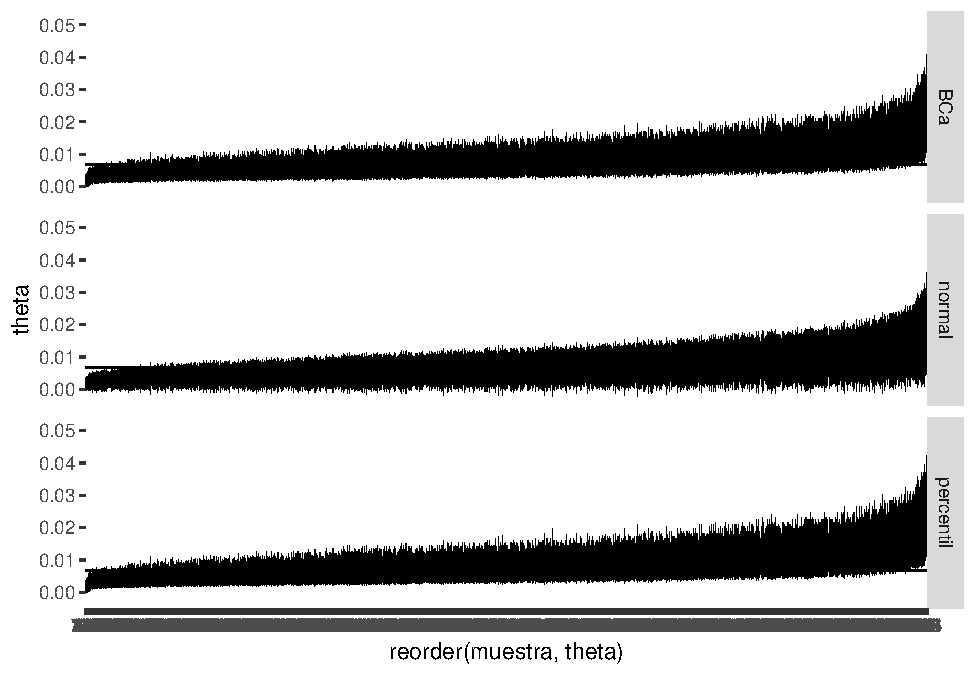
\includegraphics{ExamenParcial_files/figure-latex/poisson grafica-1.pdf}

\begin{enumerate}
\def\labelenumi{\alph{enumi})}
\setcounter{enumi}{2}
\tightlist
\item
  Repite los incisos a) y b) seleccionando muestras de tamaño \(300\).
\end{enumerate}

Primero hacemos las repeticiones con el tamano de muestra 300.

\begin{Shaded}
\begin{Highlighting}[]
\NormalTok{poiss_rep_int_}\DecValTok{300}\NormalTok{ <-}\StringTok{ }\KeywordTok{rerun}\NormalTok{(}\DecValTok{1000}\NormalTok{, }\KeywordTok{poiss_intervalos}\NormalTok{(}\DecValTok{300}\NormalTok{))}\OperatorTok
\StringTok{  }\KeywordTok{bind_rows}\NormalTok{(}\DataTypeTok{.id =} \StringTok{'muestra'}\NormalTok{) }\OperatorTok\StringTok{ }
\StringTok{  }\KeywordTok{mutate}\NormalTok{(}\DataTypeTok{fallo_izquierda =} \KeywordTok{exp}\NormalTok{(}\OperatorTok{-}\DecValTok{2}\OperatorTok{*}\FloatTok{2.5}\NormalTok{)}\OperatorTok{<}\NormalTok{inferior,}
         \DataTypeTok{fallo_derecha =} \KeywordTok{exp}\NormalTok{(}\OperatorTok{-}\DecValTok{2}\OperatorTok{*}\FloatTok{2.5}\NormalTok{)}\OperatorTok{>}\NormalTok{superior,}
         \DataTypeTok{Longitud =}\NormalTok{ superior}\OperatorTok{-}\NormalTok{inferior)}
\end{Highlighting}
\end{Shaded}

Así obtenemos la siguiente tabla:

\begin{Shaded}
\begin{Highlighting}[]
\NormalTok{poiss_rep_int_}\DecValTok{300} \OperatorTok\StringTok{ }
\StringTok{  }\KeywordTok{group_by}\NormalTok{(metodo) }\OperatorTok\StringTok{ }
\StringTok{  }\KeywordTok{summarise}\NormalTok{(}\DataTypeTok{P_fallo_izquierda =} \KeywordTok{sum}\NormalTok{(fallo_izquierda)}\OperatorTok{/}\KeywordTok{n}\NormalTok{(),}
            \DataTypeTok{P_fallo_derecha =} \KeywordTok{sum}\NormalTok{(fallo_derecha)}\OperatorTok{/}\KeywordTok{n}\NormalTok{(),}
            \DataTypeTok{Cobertura =} \DecValTok{1} \OperatorTok{-}\StringTok{ }\NormalTok{P_fallo_izquierda }\OperatorTok{-}\StringTok{ }\NormalTok{P_fallo_derecha,}
            \DataTypeTok{Longitud_promedio =} \KeywordTok{mean}\NormalTok{(Longitud))}\OperatorTok\StringTok{ }
\StringTok{  }\KeywordTok{kable}\NormalTok{()}
\end{Highlighting}
\end{Shaded}

\begin{longtable}[]{@{}lrrrr@{}}
\toprule
metodo & P\_fallo\_izquierda & P\_fallo\_derecha & Cobertura &
Longitud\_promedio\tabularnewline
\midrule
\endhead
BCa & 0.020 & 0.030 & 0.950 & 0.0049177\tabularnewline
normal & 0.005 & 0.050 & 0.945 & 0.0049909\tabularnewline
percentil & 0.026 & 0.027 & 0.947 & 0.0049767\tabularnewline
\bottomrule
\end{longtable}

Y la siguiente gráfica:

\begin{Shaded}
\begin{Highlighting}[]
  \KeywordTok{ggplot}\NormalTok{(poiss_rep_int_}\DecValTok{300}\NormalTok{) }\OperatorTok{+}
\StringTok{    }\KeywordTok{geom_pointrange}\NormalTok{(}\KeywordTok{aes}\NormalTok{(}\DataTypeTok{x =} \KeywordTok{reorder}\NormalTok{(muestra,theta),}
                        \DataTypeTok{ymin =}\NormalTok{ inferior,}
                        \DataTypeTok{y=}\NormalTok{theta,}
                        \DataTypeTok{ymax =}\NormalTok{ superior),}
                    \DataTypeTok{size=}\FloatTok{0.2}\NormalTok{) }\OperatorTok{+}
\StringTok{    }\KeywordTok{geom_hline}\NormalTok{(}\DataTypeTok{yintercept =} \KeywordTok{exp}\NormalTok{(}\OperatorTok{-}\FloatTok{2.5}\OperatorTok{*}\DecValTok{2}\NormalTok{)) }\OperatorTok{+}
\StringTok{    }\KeywordTok{facet_grid}\NormalTok{(metodo}\OperatorTok{~}\NormalTok{.)}
\end{Highlighting}
\end{Shaded}

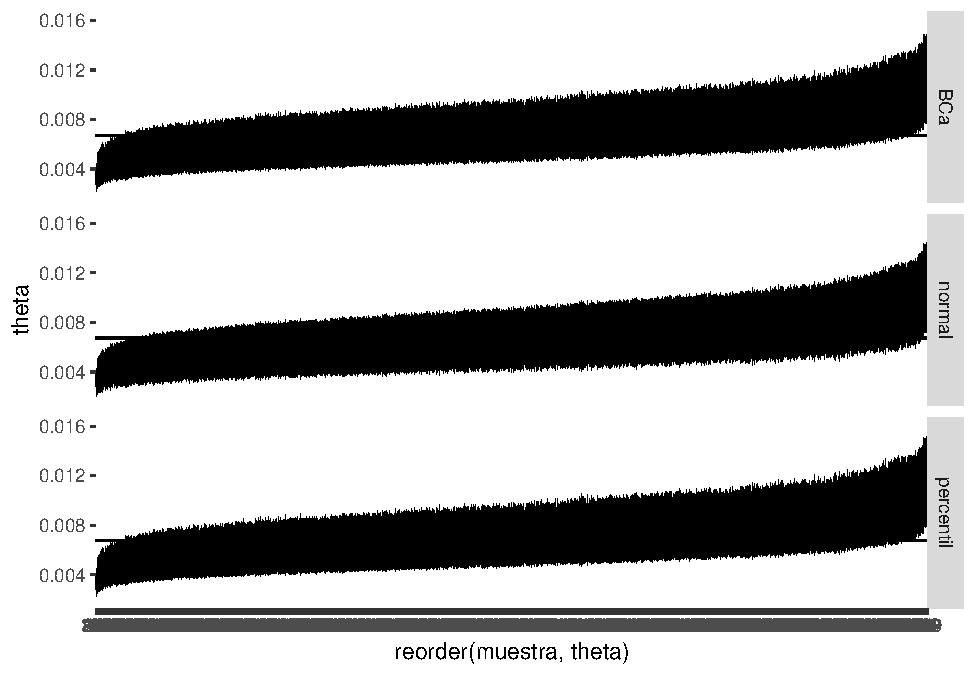
\includegraphics{ExamenParcial_files/figure-latex/poisson grafica 300-1.pdf}

Con las gráficas se ve claramente el fenómeno de la expansión y la
aceleración porque la cobertura al principio esta por debajo del
parámetro y conforme se van haciendo las replicaciones poco a poco se va
teniendo mayor cobertura del parámetro.El método de intervalos que cubre
mas es el método normal aunque al inicio tiene un porcentaje de fallo
similar al de los demás métodos.

\hypertarget{cobertura-en-la-practica}{%
\paragraph{4. Cobertura en la práctica}\label{cobertura-en-la-practica}}

En el caso del conteo rápido es posible evaluar la cobertura del
intervalo de confianza bootstrap usando los resultados de elecciones
pasadas, para ello usaremos los resultados de las elecciones 2006 (datos
\texttt{election\_2006} del paquete \texttt{estcomp}) repetirás los
siguientes dos pasos 100 veces (asegurate de que tu ejercicio de
simulación sea replicable):

\begin{enumerate}
\def\labelenumi{\arabic{enumi}.}
\tightlist
\item
  Selecciona una muestra estratificada de \texttt{election\_2006} usando
  los tamaños de muestra que indica la tabla
  \texttt{strata\_sample\_2006} (donde \texttt{n} era el tamaño de
  muestra por estrato y \texttt{N} es el número de casillas en el
  mismo).
\end{enumerate}

Para elegir la muestra se define la siguiente funcion:

\begin{Shaded}
\begin{Highlighting}[]
\NormalTok{muestra_}\DecValTok{2006}\NormalTok{ <-}\StringTok{ }\ControlFlowTok{function}\NormalTok{(}\DataTypeTok{df=}\NormalTok{election_}\DecValTok{2006}\NormalTok{)\{}
\NormalTok{  df }\OperatorTok\StringTok{ }
\StringTok{    }\KeywordTok{select}\NormalTok{(stratum,pri_pvem,pan,panal,prd_pt_conv,psd,otros) }\OperatorTok\StringTok{ }
\StringTok{    }\KeywordTok{left_join}\NormalTok{(strata_sample_}\DecValTok{2006}\NormalTok{) }\OperatorTok
\StringTok{    }\KeywordTok{split}\NormalTok{(.}\OperatorTok{$}\NormalTok{stratum) }\OperatorTok\StringTok{ }
\StringTok{    }\KeywordTok{map_df}\NormalTok{(}\OperatorTok{~}\KeywordTok{sample_n}\NormalTok{(., }\DataTypeTok{size=}\KeywordTok{first}\NormalTok{(.}\OperatorTok{$}\NormalTok{n)))}
\NormalTok{\}}
\end{Highlighting}
\end{Shaded}

\begin{enumerate}
\def\labelenumi{\arabic{enumi}.}
\setcounter{enumi}{1}
\tightlist
\item
  Utiliza estimador de razón y bootstrap para construir intervalos de
  confianza para todos los candidatos.
\end{enumerate}

Primer construimos una función para obtener el estimador de razón:

\begin{Shaded}
\begin{Highlighting}[]
\NormalTok{estimador_razon <-}\StringTok{ }\ControlFlowTok{function}\NormalTok{(df)\{}
\NormalTok{  df }\OperatorTok
\StringTok{    }\KeywordTok{pivot_longer}\NormalTok{(pri_pvem}\OperatorTok{:}\NormalTok{otros, }\DataTypeTok{names_to =} \StringTok{'partido'}\NormalTok{, }\DataTypeTok{values_to =} \StringTok{'votos'}\NormalTok{) }\OperatorTok\StringTok{ }
\StringTok{    }\KeywordTok{mutate}\NormalTok{(}\DataTypeTok{v_total =}\NormalTok{ N}\OperatorTok{*}\NormalTok{votos}\OperatorTok{/}\NormalTok{n, }\DataTypeTok{total =} \KeywordTok{sum}\NormalTok{(v_total)) }\OperatorTok\StringTok{ }
\StringTok{    }\KeywordTok{group_by}\NormalTok{(partido) }\OperatorTok\StringTok{ }
\StringTok{    }\KeywordTok{summarise}\NormalTok{(}\DataTypeTok{p=}\KeywordTok{sum}\NormalTok{(v_total)}\OperatorTok{/}\KeywordTok{mean}\NormalTok{(total)) }\OperatorTok\StringTok{ }
\StringTok{    }\KeywordTok{pivot_wider}\NormalTok{(}\DataTypeTok{names_from =}\NormalTok{ partido, }\DataTypeTok{values_from =}\NormalTok{ p)}
\NormalTok{\}}
\end{Highlighting}
\end{Shaded}

Ayudándonos de esta función, se construye una fución para obtener el
estimador bootstrap:

\begin{Shaded}
\begin{Highlighting}[]
\NormalTok{elecciones_boot <-}\StringTok{ }\ControlFlowTok{function}\NormalTok{(}\DataTypeTok{df=}\NormalTok{muestra)\{}
\NormalTok{  muestra_boot <-}\StringTok{ }\NormalTok{df }\OperatorTok\StringTok{ }
\StringTok{    }\KeywordTok{group_by}\NormalTok{(stratum) }\OperatorTok
\StringTok{    }\KeywordTok{sample_frac}\NormalTok{(}\DataTypeTok{size =} \DecValTok{1}\NormalTok{, }\DataTypeTok{replace =} \OtherTok{TRUE}\NormalTok{) }\OperatorTok\StringTok{ }
\StringTok{    }\KeywordTok{ungroup}\NormalTok{()}
    \KeywordTok{estimador_razon}\NormalTok{(muestra_boot)}
\NormalTok{\}}
\end{Highlighting}
\end{Shaded}

Asi, podemos obtener una distribucion bootstrap

\begin{Shaded}
\begin{Highlighting}[]
\NormalTok{muestra1 <-}\StringTok{ }\KeywordTok{muestra_2006}\NormalTok{()}
\NormalTok{elecciones_muestras_boot <-}\StringTok{ }\KeywordTok{rerun}\NormalTok{(}\DecValTok{1000}\NormalTok{,}\KeywordTok{elecciones_boot}\NormalTok{(muestra1)) }\OperatorTok\StringTok{ }\KeywordTok{bind_rows}\NormalTok{()}
\end{Highlighting}
\end{Shaded}

Y con esto el intervalo de confianza:

\begin{Shaded}
\begin{Highlighting}[]
\NormalTok{elecciones_pi <-}\StringTok{ }\KeywordTok{estimador_razon}\NormalTok{(muestra1)}
\NormalTok{elecciones_es <-}\StringTok{ }\KeywordTok{map_dbl}\NormalTok{(elecciones_muestras_boot,sd)}
\KeywordTok{rbind}\NormalTok{(}\DataTypeTok{razon =}\NormalTok{ elecciones_pi) }\OperatorTok\StringTok{ }
\StringTok{  }\KeywordTok{rbind}\NormalTok{(}\DataTypeTok{inferior =}\NormalTok{ elecciones_pi }\OperatorTok{+}\StringTok{ }\NormalTok{elecciones_es}\OperatorTok{*}\KeywordTok{qnorm}\NormalTok{(}\FloatTok{0.025}\NormalTok{)) }\OperatorTok\StringTok{ }
\StringTok{  }\KeywordTok{rbind}\NormalTok{(}\DataTypeTok{superior =}\NormalTok{elecciones_pi }\OperatorTok{+}\StringTok{ }\NormalTok{elecciones_es}\OperatorTok{*}\KeywordTok{qnorm}\NormalTok{(}\FloatTok{0.975}\NormalTok{)) }\OperatorTok\StringTok{ }
\StringTok{  }\KeywordTok{t}\NormalTok{()}
\end{Highlighting}
\end{Shaded}

\begin{verbatim}
##                   razon    inferior   superior
## otros       0.028630387 0.028219566 0.02904121
## pan         0.358575842 0.355941574 0.36121011
## panal       0.009958717 0.009630307 0.01028713
## prd_pt_conv 0.352538506 0.350208144 0.35486887
## pri_pvem    0.223109441 0.221150183 0.22506870
## psd         0.027187107 0.026838376 0.02753584
\end{verbatim}

Evalúa la cobertura del intervalo para cada candidato a lo largo de las
100 muestras, presenta los resultados en una tabla que incluya la
longitud media de los intervalos y la cobertura observada.

Para hacer las 100 repeticiones, definimos la funcion siguiente:

\begin{Shaded}
\begin{Highlighting}[]
\NormalTok{elecciones_boot_rep <-}\StringTok{ }\ControlFlowTok{function}\NormalTok{(}\DataTypeTok{df=}\NormalTok{election_}\DecValTok{2006}\NormalTok{)\{}
\NormalTok{  muestra <-}\StringTok{ }\KeywordTok{muestra_2006}\NormalTok{(df)}
\NormalTok{  razon_pi <-}\StringTok{ }\KeywordTok{estimador_razon}\NormalTok{(muestra)}
\NormalTok{  muestras_boot <-}\StringTok{ }\KeywordTok{rerun}\NormalTok{(}\DecValTok{1000}\NormalTok{,}\KeywordTok{elecciones_boot}\NormalTok{(muestra)) }\OperatorTok\StringTok{ }\KeywordTok{bind_rows}\NormalTok{()}
\NormalTok{  error <-}\StringTok{ }\KeywordTok{map_dbl}\NormalTok{(muestras_boot,sd)}
  
  \KeywordTok{rbind}\NormalTok{(}\DataTypeTok{razon=}\NormalTok{razon_pi) }\OperatorTok\StringTok{ }
\StringTok{    }\KeywordTok{rbind}\NormalTok{(}\DataTypeTok{inferior =}\NormalTok{ razon_pi}\OperatorTok{+}\NormalTok{error}\OperatorTok{*}\KeywordTok{qnorm}\NormalTok{(}\FloatTok{0.025}\NormalTok{)) }\OperatorTok\StringTok{ }
\StringTok{    }\KeywordTok{rbind}\NormalTok{(}\DataTypeTok{superior =}\NormalTok{ razon_pi}\OperatorTok{+}\NormalTok{error}\OperatorTok{*}\KeywordTok{qnorm}\NormalTok{(}\FloatTok{0.975}\NormalTok{)) }\OperatorTok\StringTok{ }
\StringTok{    }\KeywordTok{t}\NormalTok{() }\OperatorTok\StringTok{ }
\StringTok{    }\KeywordTok{as.data.frame}\NormalTok{() }\OperatorTok\StringTok{ }
\StringTok{    }\KeywordTok{rownames_to_column}\NormalTok{(}\StringTok{'partido'}\NormalTok{)}
    
\NormalTok{\}}
\end{Highlighting}
\end{Shaded}

Con esta funcion corremos las 100 repeticiones:

\begin{Shaded}
\begin{Highlighting}[]
\NormalTok{elecciones_repeticiones <-}\StringTok{ }\KeywordTok{rerun}\NormalTok{(}\DecValTok{100}\NormalTok{, }\KeywordTok{elecciones_boot_rep}\NormalTok{()) }\OperatorTok\StringTok{ }
\StringTok{  }\KeywordTok{bind_rows}\NormalTok{(}\DataTypeTok{.id =} \StringTok{'repeticion'}\NormalTok{)}
\end{Highlighting}
\end{Shaded}

Los resultados se presentan en la siguiente tabla:

\begin{Shaded}
\begin{Highlighting}[]
\NormalTok{elecciones_repeticiones }\OperatorTok\StringTok{ }
\KeywordTok{mutate}\NormalTok{(}\DataTypeTok{fallo_izquierda =}\NormalTok{ razon}\OperatorTok{<}\NormalTok{inferior,}
       \DataTypeTok{fallo_derecha =}\NormalTok{ superior}\OperatorTok{<}\NormalTok{razon,}
       \DataTypeTok{longitud =}\NormalTok{ superior}\OperatorTok{-}\NormalTok{inferior) }\OperatorTok\StringTok{ }
\KeywordTok{group_by}\NormalTok{(partido) }\OperatorTok\StringTok{ }
\KeywordTok{summarise}\NormalTok{(}\DataTypeTok{fallo_izquierda =} \KeywordTok{sum}\NormalTok{(fallo_izquierda)}\OperatorTok{/}\KeywordTok{n}\NormalTok{(),}
          \DataTypeTok{fallo_derecha =} \KeywordTok{sum}\NormalTok{(fallo_derecha)}\OperatorTok{/}\KeywordTok{n}\NormalTok{(),}
          \DataTypeTok{cobertura =} \DecValTok{1} \OperatorTok{-}\StringTok{ }\NormalTok{fallo_izquierda }\OperatorTok{-}\StringTok{ }\NormalTok{fallo_derecha,}
          \DataTypeTok{longitud =} \KeywordTok{mean}\NormalTok{(longitud)) }\OperatorTok\StringTok{ }
\StringTok{  }\KeywordTok{kable}\NormalTok{(}\DataTypeTok{round =} \DecValTok{4}\NormalTok{)}
\end{Highlighting}
\end{Shaded}

\begin{longtable}[]{@{}lrrrr@{}}
\toprule
partido & fallo\_izquierda & fallo\_derecha & cobertura &
longitud\tabularnewline
\midrule
\endhead
otros & 0 & 0 & 1 & 0.0010367\tabularnewline
pan & 0 & 0 & 1 & 0.0052655\tabularnewline
panal & 0 & 0 & 1 & 0.0005689\tabularnewline
prd\_pt\_conv & 0 & 0 & 1 & 0.0046776\tabularnewline
pri\_pvem & 0 & 0 & 1 & 0.0039224\tabularnewline
psd & 0 & 0 & 1 & 0.0006787\tabularnewline
\bottomrule
\end{longtable}

\textbf{Opicional (punto extra):} Las muestras con las que se estima en
el conteo rápido nunca llegan completas, y los faltantes suelen
presentar patrones, por ejemplo, las casillas en las zonas rurales
tienen mayor probabilidad de no llegar. Repite el ejercicio de
simulación de arriba añadiendo un paso de casillas faltantes, lo que
debes hacer es que una vez simulada una muestra \emph{completa} cada
casilla se censura de acuerdo a cierta probabilidad (tu la eliges como
desees), y esta probabilidad puede depender, por ejemplo, de si la
casilla es rural o urbana o quizá puede variar por estado. Elige uno (o
más) procedimiento(s) de censura de casillas y evalúa la cobertura de
los intervalos en este(os) escenario(s). Puedes explorar las variables
disponibles viendo la documentación de los datos
(\texttt{?election\_2006}).

\hypertarget{simulacion-de-variables-aleatorias}{%
\paragraph{5. Simulación de variables
aleatorias}\label{simulacion-de-variables-aleatorias}}

Recuerda que una variable aleatoria \(X\) tiene una distribución
geométrica con parámetro \(p\) si \[p_X(i) = P(X=i)=pq^{i-1}\] para
\(i=1,2,...\) y donde \(q=1-p\).

Notemos que \[\sum_{i=1}^{j-1}P(X=i)=1-P(X\geq j-1)\] \[=1 - q^{j-1}\]
para \(j\geq 1\). por lo que podemos generar un valor de \(X\) generando
un número aleatorio \(U\) y seleccionando \(j\) tal que
\[1-q^{j-1} \leq U \leq 1-q^j\]

Esto es, podemos definir \(X\) como: \[X=min\{j : (1-p)^j < 1-U\}\]
usando que el logaritmo es una función monótona (i.e.~\(a<b\) implica
\(log(a)<log(b)\)) obtenemos que podemos expresar \(X\) como
\[X=min\big\{j : j \cdot log(q) < log(1-U)\big\}\]
\[=min\big\{j : j > log(U)/log(q)\big\}\] entonces
\[X= int\bigg(\frac{log(U)}{log(q)}\bigg)+1\]

es geométrica con parámetro \(p\).

Ahora, sea \(X\) el número de lanzamientos de una moneda que se
requieren para alcanzar \(r\) éxitos (soles) cuando cada lanzamiento es
independiente, \(X\) tiene una distribución binomial negativa.

Una variable aleatoria \(X\) tiene distribución binomial negativa con
parámetros \((r,p)\) donde \(r\) es un entero positivo y \(0<p<r\) si
\[P(X=j)=\frac{(j-1)!}{(j-r)!(r-1)!}p^r(1-p)^{j-r}.\]

\begin{enumerate}
\def\labelenumi{\alph{enumi})}
\tightlist
\item
  Recuerda la distribución geométrica ¿cuál es a relación entre la
  variable aleatoria binomial negativa y la geométrica?
\end{enumerate}

La distribución geometrica es un caso particular de la binomian negativa
cuando \(r=1\), es decir, cuando solo se quiere obtener el número de
lanzamientos antes del primer exito.

\begin{enumerate}
\def\labelenumi{\alph{enumi})}
\setcounter{enumi}{1}
\tightlist
\item
  Utiliza el procedimiento descrito para generar observaciones de una
  variable aleatoria con distribución geométrica y la relación entre la
  geométrica y la binomial negativa para generar simulaciones de una
  variable aleatoria con distribución binomial negativa (parámetro p =
  0.7, r = 20). Utiliza la semilla 341285 y reporta las primeras 10
  simulaciones obtenidas.
\end{enumerate}

Para el caso de la geometrica usamos directamente la fórmula.

\begin{Shaded}
\begin{Highlighting}[]
\KeywordTok{set.seed}\NormalTok{(}\DecValTok{341285}\NormalTok{)}
\NormalTok{sim_geometrica <-}\StringTok{ }\ControlFlowTok{function}\NormalTok{(p, }\DataTypeTok{n=}\DecValTok{1}\NormalTok{)\{}
\NormalTok{  U <-}\StringTok{ }\KeywordTok{runif}\NormalTok{(n)}
\NormalTok{  q <-}\StringTok{ }\NormalTok{(}\DecValTok{1}\OperatorTok{-}\NormalTok{p)}
  \KeywordTok{as.integer}\NormalTok{(}\KeywordTok{log}\NormalTok{(U)}\OperatorTok{/}\KeywordTok{log}\NormalTok{(q))}\OperatorTok{+}\DecValTok{1}
\NormalTok{\}}

\KeywordTok{sim_geometrica}\NormalTok{(}\FloatTok{0.7}\NormalTok{,}\DecValTok{10}\NormalTok{)  }
\end{Highlighting}
\end{Shaded}

\begin{verbatim}
##  [1] 1 1 1 1 2 2 1 1 2 1
\end{verbatim}

Dado que la binomial negativa se puede ver como una serie de
geométricas, hasta juntar el número de éxitos \emph{k} deseados, puede
usarse la función definida arriba para simular la binomial negativa. De
esta manera tenemos::

\begin{Shaded}
\begin{Highlighting}[]
\NormalTok{sim_binn <-}\StringTok{ }\ControlFlowTok{function}\NormalTok{(p,r)\{}
  \KeywordTok{sum}\NormalTok{(}\KeywordTok{sim_geometrica}\NormalTok{(p,}\DataTypeTok{n=}\NormalTok{r))}
\NormalTok{\}}

\KeywordTok{rerun}\NormalTok{(}\DecValTok{10}\NormalTok{,}\KeywordTok{sim_binn}\NormalTok{(}\FloatTok{0.7}\NormalTok{,}\DecValTok{20}\NormalTok{)) }\OperatorTok\StringTok{ }\KeywordTok{flatten_dbl}\NormalTok{()}
\end{Highlighting}
\end{Shaded}

\begin{verbatim}
##  [1] 25 28 28 31 29 35 34 30 29 30
\end{verbatim}

\begin{enumerate}
\def\labelenumi{\alph{enumi})}
\setcounter{enumi}{2}
\tightlist
\item
  Verifica la relación \[p_{j+1}=\frac{j(1-p)}{j+1-r}p_j\]
\end{enumerate}

y úsala para generar un nuevo algoritmo de simulación, vuelve a definir
la semilla y reporta las primeras 10 simulaciones.

\[ \frac{p_{j +1}}{p_j} = \frac{\frac{j!}{(j+1-r)!(r-1)!}p^r(1-p)^{j+1-r}}{\frac{(j-1)!}{(j-r)!(r-1)!}p^r(1-p)^{j-r}}= \frac{j(1 - p) }{j + 1 - r}.\]

Usando esta relación recursiba es posible construir un algoritmo similar
al \emph{poisson} visto en clase, el cual se esperaría fera más
eficiente al definido usando la relación entre geométrica y binomial
negativa.

\begin{Shaded}
\begin{Highlighting}[]
\KeywordTok{set.seed}\NormalTok{(}\DecValTok{341285}\NormalTok{)}
\NormalTok{sim_binn_rec <-}\StringTok{ }\ControlFlowTok{function}\NormalTok{(p,r)\{}
\NormalTok{  U <-}\StringTok{ }\KeywordTok{runif}\NormalTok{(}\DecValTok{1}\NormalTok{)}
\NormalTok{  i <-}\StringTok{ }\NormalTok{r}
\NormalTok{  f <-}\StringTok{ }\NormalTok{p}\OperatorTok{^}\NormalTok{r}
\NormalTok{  P <-}\StringTok{ }\NormalTok{f}
  \ControlFlowTok{while}\NormalTok{(U}\OperatorTok{>=}\NormalTok{P)\{}
\NormalTok{    f <-}\StringTok{ }\NormalTok{i}\OperatorTok{*}\NormalTok{(}\DecValTok{1}\OperatorTok{-}\NormalTok{p)}\OperatorTok{*}\NormalTok{f}\OperatorTok{/}\NormalTok{(i}\OperatorTok{+}\DecValTok{1}\OperatorTok{-}\NormalTok{r)}
\NormalTok{    P <-}\StringTok{ }\NormalTok{P}\OperatorTok{+}\NormalTok{f}
\NormalTok{    i <-}\StringTok{ }\NormalTok{i}\OperatorTok{+}\DecValTok{1}
\NormalTok{  \}}
\NormalTok{  i}
\NormalTok{\}}

\KeywordTok{rerun}\NormalTok{(}\DecValTok{10}\NormalTok{, }\KeywordTok{sim_binn_rec}\NormalTok{(}\FloatTok{0.7}\NormalTok{,}\DecValTok{20}\NormalTok{)) }\OperatorTok\StringTok{ }\KeywordTok{flatten_dbl}\NormalTok{()}
\end{Highlighting}
\end{Shaded}

\begin{verbatim}
##  [1] 30 29 31 30 26 25 33 27 25 40
\end{verbatim}

\begin{enumerate}
\def\labelenumi{\alph{enumi})}
\setcounter{enumi}{3}
\tightlist
\item
  Realiza 10,000 simulaciones usando cada uno de los algoritmos y
  compara el tiempo de ejecución (puedes usar la función
  \texttt{system.time()}.
\end{enumerate}

\begin{Shaded}
\begin{Highlighting}[]
\KeywordTok{system.time}\NormalTok{(}\KeywordTok{rerun}\NormalTok{(}\DecValTok{10000}\NormalTok{, }\KeywordTok{sim_binn}\NormalTok{(}\FloatTok{0.7}\NormalTok{,}\DecValTok{20}\NormalTok{)))}
\end{Highlighting}
\end{Shaded}

\begin{verbatim}
##    user  system elapsed 
##    0.08    0.00    0.08
\end{verbatim}

\begin{Shaded}
\begin{Highlighting}[]
\KeywordTok{system.time}\NormalTok{(}\KeywordTok{rerun}\NormalTok{(}\DecValTok{10000}\NormalTok{, }\KeywordTok{sim_binn_rec}\NormalTok{(}\FloatTok{0.7}\NormalTok{,}\DecValTok{20}\NormalTok{)))}
\end{Highlighting}
\end{Shaded}

\begin{verbatim}
##    user  system elapsed 
##    0.08    0.00    0.08
\end{verbatim}

Como se esperaba, en la función recursiva de la binomial el tiempo de
ejecución es menor por el while que tiene la función, ya que solo
calcula en función al valor de \(U\), sin hacer cálculos innecesarios.

\begin{enumerate}
\def\labelenumi{\alph{enumi})}
\setcounter{enumi}{4}
\tightlist
\item
  Genera un histogrma para cada algoritmo (usa 1000 simulaciones) y
  comparalo con la distribución construida usando la función de R
  \emph{dnbinom}.
\end{enumerate}

\begin{Shaded}
\begin{Highlighting}[]
\NormalTok{binn_alg1 <-}\StringTok{ }\KeywordTok{rerun}\NormalTok{(}\DecValTok{10000}\NormalTok{, }\KeywordTok{sim_binn}\NormalTok{(}\FloatTok{0.7}\NormalTok{,}\DecValTok{20}\NormalTok{)) }\OperatorTok\StringTok{ }\KeywordTok{flatten_dbl}\NormalTok{()}
\NormalTok{binn_alg2 <-}\StringTok{ }\KeywordTok{rerun}\NormalTok{(}\DecValTok{10000}\NormalTok{, }\KeywordTok{sim_binn_rec}\NormalTok{(}\FloatTok{0.7}\NormalTok{,}\DecValTok{20}\NormalTok{))}\OperatorTok\StringTok{ }\KeywordTok{flatten_dbl}\NormalTok{()}
\NormalTok{binn_R <-}\StringTok{ }\NormalTok{(}\KeywordTok{rnbinom}\NormalTok{(}\DecValTok{10000}\NormalTok{, }\DataTypeTok{size =} \DecValTok{20}\NormalTok{, }\DataTypeTok{p =} \FloatTok{0.7}\NormalTok{)}\OperatorTok{+}\DecValTok{20}\NormalTok{)}

\NormalTok{binn_hist <-}\StringTok{ }\KeywordTok{tibble}\NormalTok{(}\DataTypeTok{Alg1 =}\NormalTok{ binn_alg1,}
                        \DataTypeTok{Alg2 =}\NormalTok{ binn_alg2,}
                        \DataTypeTok{R =}\NormalTok{ binn_R) }\OperatorTok\StringTok{ }
\StringTok{  }\KeywordTok{pivot_longer}\NormalTok{(Alg1}\OperatorTok{:}\NormalTok{R,}\DataTypeTok{names_to =} \StringTok{'modelo'}\NormalTok{, }\DataTypeTok{values_to =} \StringTok{'valor'}\NormalTok{)}

\KeywordTok{ggplot}\NormalTok{(binn_hist) }\OperatorTok{+}\StringTok{ }
\StringTok{  }\KeywordTok{geom_histogram}\NormalTok{(}\KeywordTok{aes}\NormalTok{(valor), }\DataTypeTok{breaks =} \DecValTok{20}\OperatorTok{:}\DecValTok{45}\NormalTok{) }\OperatorTok{+}
\StringTok{  }\KeywordTok{facet_grid}\NormalTok{(modelo}\OperatorTok{~}\NormalTok{.) }\OperatorTok{+}
\StringTok{  }\KeywordTok{theme_light}\NormalTok{()}
\end{Highlighting}
\end{Shaded}

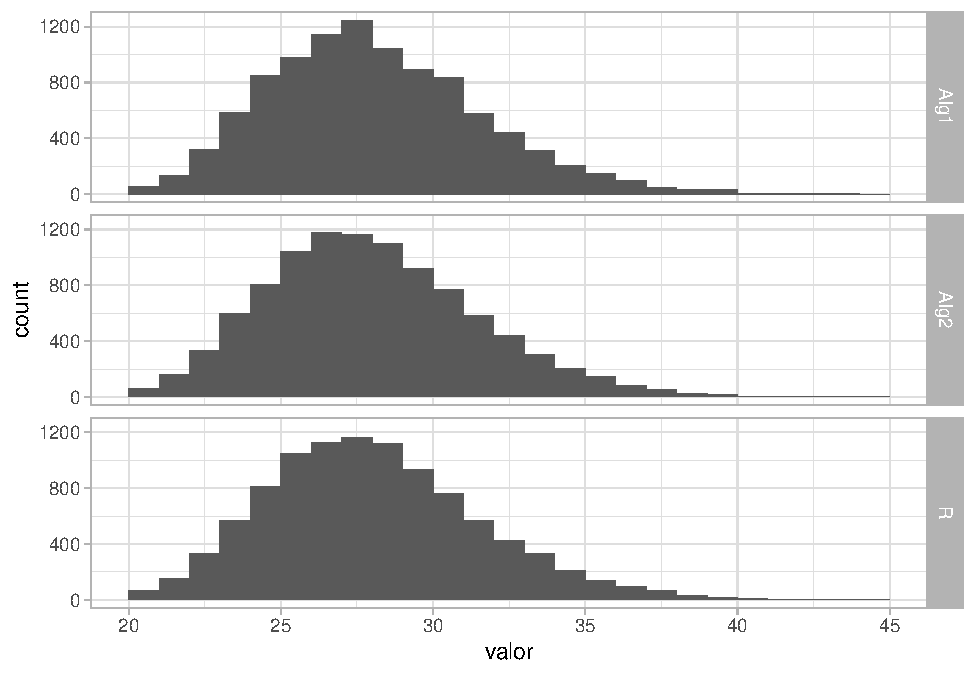
\includegraphics{ExamenParcial_files/figure-latex/binneg histograma-1.pdf}

Los tres algormitmos arrogan resultados muy similares, por lo que
posiblemente la diferencia sea la eficiencia de cómputo.


\end{document}
